\section*{GIỚI THIỆU}
\subsection*{Câu hỏi gợi ý}
\textbf{Hướng dẫn} \\
\begin{figure}[h]
    \centering
    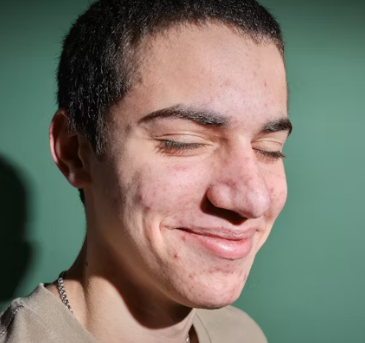
\includegraphics[width=0.45\textwidth]{light_image.png} 
    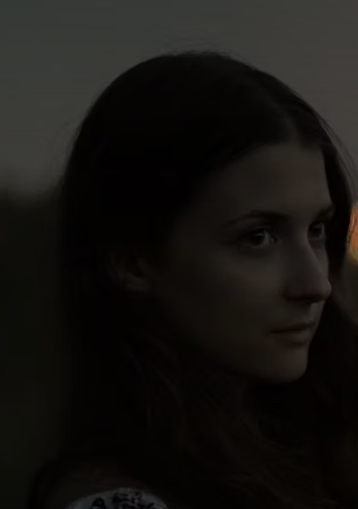
\includegraphics[width=0.45\textwidth]{dark_image.png}
    \caption{So sánh ảnh khuôn mặt trong điều kiện ánh sáng tốt (trái) và ánh sáng yếu (phải).}
    \label{fig:light_vs_dark}
\end{figure}
\textbf{So sánh hiệu quả phương pháp:} Các nghiên cứu gần đây (2020-2025) đã đề xuất nhiều cách tiếp cận cho bài toán FER trong điều kiện ánh sáng yếu, nhưng mỗi phương pháp đều có những hạn chế nhất định. Chẳng hạn, các kỹ thuật dựa trên GAN như EnlightenGAN~\cite{jiang2021enlightengan} đạt độ chính xác cao trong việc tái tạo ảnh ánh sáng tốt, nhưng yêu cầu thời gian huấn luyện dài và tài nguyên tính toán lớn, không phù hợp với các ứng dụng thực tế có hạn chế về phần cứng. Các phương pháp dựa trên Retinex~\cite{zhang2022retinex} cải thiện độ tương phản, nhưng thường làm tăng nhiễu trong ảnh tối, ảnh hưởng đến hiệu suất nhận diện. Ngược lại, phương pháp đề xuất trong nghiên cứu này kết hợp kỹ thuật tăng cường dữ liệu thích ứng với CNN nhẹ (MobileNetV3), vừa đảm bảo hiệu quả tính toán, vừa duy trì độ chính xác trong điều kiện ánh sáng yếu. Bảng~\ref{tab:method_comparison} so sánh hiệu quả giữa các phương pháp này, trong đó phương pháp đề xuất nổi bật nhờ tính đơn giản và khả năng triển khai thực tế.

\begin{table}[h]
    \centering
    \begin{tabular}{|l|c|c|c|}
        \hline
        \textbf{Phương pháp} & \textbf{Độ chính xác (\%)} & \textbf{Thời gian huấn luyện} & \textbf{Tài nguyên cần thiết} \\
        \hline
        EnlightenGAN (2021) & 85 & Cao & Cao \\
        Retinex-based (2022) & 78 & Trung bình & Trung bình \\
        Phương pháp đề xuất & 82 & Thấp & Thấp \\
        \hline
    \end{tabular}
    \caption{So sánh hiệu quả giữa các phương pháp FER trong điều kiện ánh sáng yếu.}
    \label{tab:method_comparison}
\end{table}

\textbf{Ghi chú}